\documentclass[../main.tex]{subfiles}
\begin{document}

\chapter{Lecture 11 - 20-04-2020}

\section{Analysis of $\knn$}
$$
\barra{E} \left[{\ell_D} (\hat{\ell}_s ) \right] \leq 2 \cdot \ell_D \left( f^* \right) + c \cdot \barra{E}\left[ \, \| X = x_{\Pi(s,x)} \| \, \right]
$$
At which rate this thing goes down? If number of dimension goes up then a lot of point are far away from $X$. \\
So this quantity must depend on the space in which X live.
\\ Some dependence on number of depends and incresaing number of traning points close to $X$\\
This expecation is fucniton of random variable X and $X_{\pi(s,x)}$
\\\\
We are going to use the assumption that:
\\
$| X_t | \leq 1 \qquad \forall $ cordinates $i = 1, ..., d$
\\
\begin{figure}[h]
    \centering
    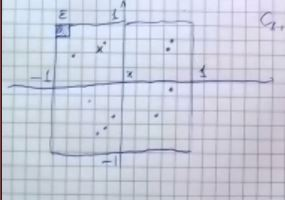
\includegraphics[width=0.6\linewidth]{../img/lez11-img1.JPG}
    \caption{Example of domain of $\knn$}
    %\label{fig:}
\end{figure}\\
\\
Hyper box in bydimension. All point live in this box and we exploit that.
Look at the little suare in which is divided and we assume that we are dividing the box in small boxes of size $\varepsilon$. Now the training points will be a strincle of point distributed in the big square. \\
Our training points are distribuited in the box (this is our S).
\\
Now we added a point x and given this two things can happned:
falls in the square with training points or in a square without training points.
\\
What is going to be the distance $X_{\pi(s,x)}$ in this two cases?
\\
We have $c_1$ up to $c_r$
How big is this when we have this two cases?
(We lookjing at specific choices of x and s)
\\
$$
\| X - X_{s,x} \| \leq \
\begin{cases}
\varepsilon \ \sqrt[]{d} \qquad C_i \cup S \neq 0 \\
\sqrt[]{d} \qquad C_i \cup S = 0
\end{cases}
$$
were $X \in C_i$
\\
We have to multiply by the lenght of the cube.
Will be $\varepsilon  \ \, \sqrt[]{d}$
\\
\begin{figure}[h]
    \centering
    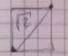
\includegraphics[width=0.1\linewidth]{../img/lez11-img2.JPG}
    \caption{Diagonal length}
    %\label{fig:}
\end{figure}\\
\\
If things go badly can be very far away like the length of the domain.
Lenght is $2$ and diagonal is $ \ \sqrt[]{d}$
\\
if close they are going to be $\varepsilon close$ or far as domain.
\\
We can split that the expression inside the expectation according to the two cases.
\\
$$
\barra{E} \left[ \, \| X - X_{\Pi(s,x)} \| \, \right] 
\leq 
$$
$$
\barra{E} \left[ 
\varepsilon \cdot \sqrt[]{d} \cdot \sum_{i = 1}^{r} I \{ X \in C_i \}
\cdot 
I \{ C_i\cap S \neq 0 \} 
\right] 
+ \ 2 \, \cdot \
\sqrt[]{d} \, \cdot \,
\sum_{i=1}^{r} I \{ X \in C_i \} 
\cdot I\{C_i \cap S \neq 0 \} 
 =
$$

$$
= \varepsilon \cdot \ \sqrt[]{d} \cdot \ \barra{E} \left[ \, 
\bred{ $
\sum_{t = 1}^{r} I \{ X \in C_i \} I \cdot  \{C_i \cap S \neq 0 \}   $}\,  \right]
 + 2 \cdot \ \sqrt[]{d}\  \cdot \ \sum_{i = 1}^{r} 
\barra{E} \left[ \,
I \{ X \in C_1 \} 
\cdot 
I \{ C_1 \cap S \neq 0 \} \,
\right] \leq
$$
I don't care about this one \red{$\sum_{t = 1}^{r} I \{ X \in C_i \}\cdot I  
\{ C_i \cap S \neq 0 \}  $} 
\\
Can be either $0$ or $1$ (if for some $i$, $X$ belong to some $C_i$
\\
So at most 1 the expectation
$$
\leq \ \varepsilon \cdot \ \sqrt[]{d} + \square
$$
We can bound this square. Are the event I in the summation of the term after $+$. If they are indepednt the product will be the product of the two expectation. If I fix the cube.
$X$ and $S$ are independent.
\\
Now the two events are independent \\ \bred{ $X \in C_i$ is independent of $C_i \cap S \neq $}

$$
\barra{E} 
\left[ 
\ I \{ X \in C_i \}
\cdot  
I \{ C_i \cap S \neq 0 \} 
\right] 
= \barra{E} 
\left[ 
I \{ X \in C_i \} 
\right] 
\cdot 
\barra{E} 
\left[ I \{ C_i \right \} ]
$$

MANCAAAAAAA 9.26
\\
$$
\barra{P} \left( C_i \cap S \right)  = \left( 1- \barra{P} \left( X \in C_1 \right) \right)^m \leq \exp (- m \cdot \barra{P} (x \in C_1 ))
$$
The probability of the point fall there and will be the probability of falling in the cube.
\\
Probability of Xs to fall in the cube with a m (samples?)
\\
Now use inequality $ (1 - p)^m \in e^{-pm}$ $\longrightarrow$ $1 + x \leq e^x$
\begin{figure}[h]
    \centering
    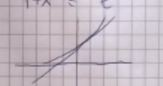
\includegraphics[width=0.2\linewidth]{../img/lez11-img3.JPG}
    \caption{Shape of the function}
    %\label{fig:}
\end{figure}\\
$$
\sum_{t = 1}^{r} \ \barra{E} \left[ \, \barra{P} \left(X \in C_1 \right) \cdot \barra{P} \left(C_1 \cap S \neq \right)\, \right] \leq \sum_{i = 1}^{r} p_i \cdot e^{-m \, p_i} \leq
$$
given that $p_i = \barra{P} (X \in C_i)$
I can upper bound this 
$$
\leq 
\sum_{t=1}^{r} 
\left(
 \max_{0 \leq p \leq 1} 
\, p \, e^{- m \, p} 
\right)
\leq
 r \, \max_{0 \leq p \leq 1} \, \red{p \, e ^{-m\,p}} \,  =
$$
where \bred{$p \, e ^{-m\,p}$} is $F(p)$
it is concave function so i'm going to take first order derivative to maximise it.
\\
$$
F'(p) = 0 \Leftrightarrow p = \frac{1}{m} \quad check!
$$
$$
F''(p) \leq 0 \qquad \qquad \qquad \qquad 
$$
Check this two condition!
$$
 = \frac{r}{e \, m}
$$
\\
Now get expectation
\\
$$
\barra{E} \left[ \, \| X - X_{\Pi(s,x)} \| \, \right] 
\leq 
\varepsilon \cdot \ \sqrt[]{d} + \left( 2 \cdot \sqrt[]{d}\right) \frac{r}{e \, m} =
$$
I have $(\frac{2}{\varepsilon})^2$ squares.
This bring $\varepsilon$ in the game
$$
\varepsilon \cdot \ \sqrt[]{d} + \left( 2 \cdot \sqrt[]{d}\right) \frac{1}{e \, m} \cdot \left( \frac{2}{\varepsilon}\right)^d = 
$$
$$
= \sqrt[]{d} \left( \varepsilon + \frac{2}{e \, m } \cdot \left( \frac{2}{\varepsilon} \right)^d \right)
$$
\blue{HE MISS THE "c" costant from the start}
we can choose $\varepsilon$ to take them balanced
\\set $\varepsilon = 2 \, m^{\frac{-1}{(d+1)}} $
\bred{ 
$$
\left( \varepsilon + \frac{2}{e \, m } \right) 
\cdot 
\left( \frac{2}{\varepsilon}^d \right) 
\leq 4 \, m ^{\frac{-1}{(d+1)}} =  
$$
}
\\
$$
\barra{E} 
\left[ 
\ell_d (\hat{h}_s)  \right] \ \
\leq \ \
2 
\ell_d (f^*)
 + 
 4 \cdot c \cdot \ \sqrt[]{d} 
 \cdot m^{- \frac{1}{d+1}}
$$
We have that:\\
if $m$ $\longrightarrow$ $\infty$ \quad 
$\ell_D (f^*) \
 \leq  \
\barra{E} \left[ \ell_D (\hat{h}_s \right] ) \ \
\leq  \ \
2 \ell_D(f^*)$
\\
I want this smaller than twice risk + some small quantity
$$
\barra{E} \left[ \ell_d(\hat{h}_S) \right] \ \leq  \ 2 \ell_D(f^*) + \varepsilon
$$
How big $m$ ?\\
Ignore this part since very small $(4 \cdot c \cdot \ \sqrt[]{•d})$
\\
$$
m ^ {-\frac{1}{d+1}} \ \leq \ \varepsilon \Leftrightarrow m \ \geq  \ \left(\frac{1}{\varepsilon}\right)^d+1 
$$
So 1-NN require a training set size exponential "accuracy" \ $1-\varepsilon$
\\\\
We show that $1-NN$ can approach twice based risk \ $2 \cdot \ell_D(f^*)$\\
but it takes a training set exponential in $d$.
\\
\subsection{Study of $\knn$}
Maybe we can use the $\knn$.
$$
\barra{E}\left[ \ell_D(\hat{h}_s)\right] \leq \left( 1+ \sqrt[]{\frac{8}{k}}\right) \ell_D(f^*) + 0 \, \left(k \, m^{-\frac{1}{d+1}}\right)
$$
So is not exponential here.
\\
\bred{Learning algorithm $A$ is consistent for a certain loss $\ell$}
\\
If $\forall \, D$(distribution) of data we have that $A(S_m)$ predictor output by $A$\\
Now have the risk of that in $\ell_D(A(S_m))$ and we look at the expectation  $\barra{E}\left[\ell_D(A(S_m))\right]$
\\If we give a training set size large ($ \ \lim_{m \rightarrow \infty} \, \barra{E}\left[\ell_D(A(S_m))\right] = \ell_D (f^*)\, $) risk will converge in based risk.
\\\\
$\knn$ where $K = K_m$ (is a function of training set size).
$K_, \rightarrow \infty $ as $m \rightarrow \infty$.
\\
Only way $K$ goes to infinity is sublinearly of training set size. (infinity but so as quicly as $m$
$K_m = O(m)$
\\\\
For instance $K_m = \sqrt[]{m}$
\\
Then: 
$$
\lim_{m \rightarrow \infty} \barra{E} \left[ \ell_D\left(A'\left(S_m\right)\right) \right] = \ell_D(f^*) \qquad \textbf{where $A'$ is $K_m$-$NN$ } 
$$
Increasing the size we will converge to this base risk for any distribution and that's nice.
\\\\
\subsection{study of trees}
Algorithm that grow tree classifiers can also be made consistent provided two condition:
\begin{itemize}
\item The tree keeps growing
\item A non-vanishing fraction of traning example is routed to each leaft
\end{itemize}
Tree has to keep growing but not so fast.\\
Second point is: suppose you have a certain number of leaves and you can look at the fraction. 
Each leaf $\ell$ gets $N_\ell$ examples. You want that this fraction at any point of time is not going to 0. The fraction of point every leaf receive a split we are reducing the smallest number of examples. 
\\Example keep growing and leaves too and we want that $\frac{N_\ell}{manca}$ this not going to 0. $.$ since not showed the formula.
\\\\
Given $A$, how do I know wheter $A$ could be consistent?
$$
H_A \equiv \{ \ h \ : \ \exists S \ A(S) = h \}
$$
$S$ can be any size.
If $A$ is $ERM$ then $H_A = H$, so where ERM minimise it.
\\
If $\exists f^* : X \longrightarrow $ such that $f^* \not\in H_A$ and $\exists D$ such that $f^*$ is Bayes optimal for some distribution $D$.\\
This cannot be consistent because distribution will not be able to generate the Bayes optimal predictor.
Maybe is there another predictor $f$ which is not equal to $f^*$ risk.
\\\\
What's the intuition?
\\Every time $A$ is such that $H_A$ is "restricted" in some sense, then $A$ cannot be consistent. (e.g $ERM$).
\\\\
Another way of restricting? Could be tree classifiers with at most $N$ nodes (bound number of nodes).
\\ How do i know $N$ is enought to approximate well $f^*$.
I want to converge the risk of $f^*$.
\\
We can introduce a class of algorithm potentially consistent in which space predictor is not restricted.
\\\\
\section{Non-parametric Algorithms}
When they are potentially consistent.
\\ What does it mean?\\
Non-parametric algorithm have the potential of being consistent and do we know if algorithm is parametric or not?
\\
$A$ is non-parametric if:
\begin{itemize}
\item the description of $A(S_m)$ grows with $m$
\end{itemize}
Your predictor is a function and let's assume i can store in any variable a real number with arbitrary precition. 
\\\\
\\\\
\bred{Any algorithm with bias is incosistent. So ability to converge to base risk is this.}
\\
How do i know if i have bias or not? this is where non parametric algorithm came.
\\
Let's consider $\knn$, how i can describe it? I have to remember distance is maded by training points and if i give you more S the m will increase. So this is parametric. 
\\
More training set for tree, then will grow more, even more larger will be ever growing more.
\\
Any algorithm as a give training points is no parametric, while growing with parametric will stop a some point.
\\
\begin{figure}[h]
    \centering
    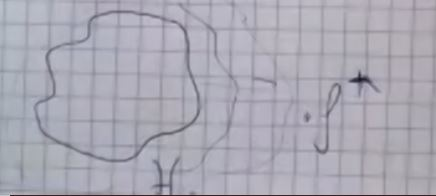
\includegraphics[width=0.5\linewidth]{../img/lez11-img4.JPG}
    \caption{Parametric  and non parametric growing as training set getting larger}
    %\label{fig:}
\end{figure}\\
\\
If algorithm is more parametric as i give training points\\
If a certain point stop growing, $f^*$ will be out and i will grow more.
\\
If algorithm is able to generate 
--- MANCA ---
Then the algorithm is non-parametric and can be potentially consistent and incluse $f^*$ as it grows.
\\
If set of predictor stops because I'm not enlarging my set of predictor since description of algortim will not depend on training size at some point \qquad $\rightarrow$ to be consistent.
\\
If bias vanashes as i increase the S, then i can be consistent. I generating predictor that description depends on how much points i give them.
\\\\
Parametric is not precise as consistency. 
\\
One class of algorithm that has consistency has a predicotr size growing with S growing.
\\
Definition of non parametric is more fuzzy, consistency is precise (we demonstrate that mathematically).
\\\\

\subsection{Example of parametric algorithms}
Neural network is parametric since i give structure of the network.
If i give S small or big S my structure will be the same (will fit better on the training points).
\\
Other example are algorithm with linear classifier in which number of parameter are just the idmension of the space.
\end{document}